% \begin{maintable}[b]
%     \centering
%     \caption{An overview of the analysis of our charting table with a count of the number of occurrences of the paper - (a) The 11 targeted human experiences in smart buildings, (b) The first 10 out of 20 design mechanisms towards enabling human experiences in smart buildings, and (c) The seven types of technological interventions developed or used by research in smart buildings.}
%     \label{tab:bigoverview}
%     \resizebox{\linewidth}{!}{%
%     \begin{tabular}{ccc}
%         (a) & (b) & (c) \\
%         \begin{tabular}[t]{ll}
%             \toprule
%             Targeted Human Experience & No. \\
%             \midrule
%             Aesthetic Experience & 18 \\
%             Bodily Experience & 23 \\
%             Comfort & 47 \\
%             Democratic Experience & 16 \\
%             Explorative and/or Future and Speculative	& 48 \\
%             Emotional Experience & 38 \\
%             Experience of Relatedness &	21 \\
%             Inclusion Experience & 13 \\
%             Learning and Teaching Experience & 9\\
%             Sense of Orientation & 8 \\
%             Sense of Place-making & 23 \\
%             \bottomrule
%         \end{tabular}
%         & 
%         \begin{tabular}[t]{ll}
%             \toprule
%             Design Mechanisms & No. \\
%             \midrule
%             Community and Social Connection & 40 \\
%             Spatial Design & 34 \\
%             Technological Immersion & 22 \\
%             Playful Design & 22 \\
%             Environmental and Social Information & 21 \\
%             Participation and Co-Design & 17 \\
%             Somaesthetic Design & 17 \\
%             Personalisation & 16 \\
%             N.A. &	12 \\
%             Biophilic Design & 9 \\
%            \multicolumn{2}{l}{...}\\
%          \bottomrule
%         \end{tabular}
%         & \begin{tabular}[t]{ll}
%             \toprule
%             Type of Technological Intervention & No. \\
%             \midrule
%             Audio and Lighting Technologies & 27\\
%             Augmented and Virtual Reality & 17 \\
%             Environmental Sensing & 23 \\
%             Feedback Systems & 11 \\
%             Interactive Displays & 45 \\ 
%             Physiological Sensing & 10 \\
%             Shape-Changing and Kinetic Interfaces & 22 \\
%             \bottomrule
%         \end{tabular}
%     \end{tabular}
%     } % END OF RESIZEBOX
% \end{maintable}

\begin{maintable}[tbp]
\centering
\caption{An overview of the analysis of our charting table with a count of the number of occurrences of the paper: (a) the 11 targeted human experiences in smart buildings, (b) the first 10 out of 20 design mechanisms towards enabling human experiences in smart buildings, and (c) the seven types of technological interventions developed or used by research in smart buildings.}
\label{tab:bigoverview}

\fontsize{7.2}{8.5}\selectfont
\setlength{\tabcolsep}{2.2pt}
\renewcommand{\arraystretch}{1.03}

\noindent
\begin{minipage}[t]{.31\linewidth}
\centering
\textbf{(a)}\par\vspace{.25\baselineskip}
\begin{tabularx}{\linewidth}{@{}Y r@{}}
\toprule
Targeted Human Experience & No. \\
\midrule
Aesthetic Experience & 18 \\
Bodily Experience & 23 \\
Comfort & 47 \\
Democratic Experience & 16 \\
Explorative and/or Future and Speculative & 48 \\
Emotional Experience & 38 \\
Experience of Relatedness & 21 \\
Inclusion Experience & 13 \\
Learning and Teaching Experience & 9 \\
Sense of Orientation & 8 \\
Sense of Place-making & 23 \\
\bottomrule
\end{tabularx}
\end{minipage}%
\hfill
\begin{minipage}[t]{.31\linewidth}
\centering
\textbf{(b)}\par\vspace{.25\baselineskip}
\begin{tabularx}{\linewidth}{@{}Y r@{}}
\toprule
Design Mechanisms & No. \\
\midrule
Community and Social Connection & 40 \\
Spatial Design & 34 \\
Technological Immersion & 22 \\
Playful Design & 22 \\
Environmental and Social Information & 21 \\
Participation and Co-Design & 17 \\
Somaesthetic Design & 17 \\
Personalisation & 16 \\
N.A. & 12 \\
Biophilic Design & 9 \\
\multicolumn{2}{@{}l@{}}{\ldots} \\
\bottomrule
\end{tabularx}
\end{minipage}%
\hfill
\begin{minipage}[t]{.31\linewidth}
\centering
\textbf{(c)}\par\vspace{.25\baselineskip}
\begin{tabularx}{\linewidth}{@{}Y r@{}}
\toprule
Type of Technological Intervention & No. \\
\midrule
Audio and Lighting Technologies & 27 \\
Augmented and Virtual Reality & 17 \\
Environmental Sensing & 23 \\
Feedback Systems & 11 \\
Interactive Displays & 45 \\
Physiological Sensing & 10 \\
Shape-Changing and Kinetic Interfaces & 22 \\
\bottomrule
\end{tabularx}
\end{minipage}

\end{maintable}

\section{Findings}
\label{sec-ch2:findings}
This section presents a descriptive overview of the literature, followed by a thematic analysis of targeted human experiences (RQ1), design mechanisms (RQ2), and technological interventions (RQ3). \autoref{tab:bigoverview} summarises the targeted human experiences (RQ1), the first 10 out of 20 identified design mechanisms (RQ2), and the technological interventions developed or applied in smart building research (RQ3).




\subsection{Characteristics of the Literature}
\label{sec-ch2:findings-descriptive}
In line with general publication increases, the distribution of the 192 papers in our corpus by publication year shows a growing trend that peaked in 2019, coinciding with the ACM ToCHI special issue on human-building interaction (HBI)~\cite{alavi2019introduction} (\autoref{fig:overview-years} in the appendix). The reviewed papers predominantly explored smart homes (24\%) or smart buildings (20\%). Smart offices (17\%) and educational spaces (15\%) also received attention, along with specific locations like places of worship, historical sites, children's play areas (19\%), and interactive installations (7\%)  (\autoref{fig:overview-building}). Publications resulted primarily from conferences (56\%) followed by journal articles (19\%), as shown in \autoref{fig:overview-publication}. Within conference publications, 22\% of works were published at ACM CHI, otherwise appearing in a variety of HCI and HCI-adjacent conferences as well as architecture and built environments conferences (\autoref{fig:overview-venue}).   


\subsection{The Targeted Human Experiences in Smart Building Research}
\label{sec-ch2:findings-experiences}
We identified 11 key themes corresponding to distinct human experiences within smart buildings, presented in \autoref{tab:bigoverview}(a). While we aimed to identify the primary and overarching human experience targeted in each paper, it was not always possible to assign works to a single experience. In those cases, papers were assigned to multiple themes. Specifically, six papers addressed three different human experiences (e.g. \cite{telhan2010interaction}), 90 targeted two (e.g. \cite{zum2022interactive}), and the remaining 96 focused on a single experience. We provide a high-level overview of the experiences below. Detailed descriptions, including the number of papers addressing each experience and prototypical examples, can be found in Tables \ref{tab:experiences} and \ref{tab:experiences2}. For readability, all targeted human experiences are in bold throughout the rest of this paper.


\begingroup
\fontsize{7.3}{8.7}\selectfont
\setlength{\tabcolsep}{2.4pt}
\renewcommand{\arraystretch}{1.04}
\setlength{\LTleft}{0pt}
\setlength{\LTright}{0pt}

\begin{longtable}{@{}%
  >{\RaggedRight\arraybackslash}p{.19\linewidth}
  >{\RaggedRight\arraybackslash}p{.39\linewidth}
  >{\centering\arraybackslash}p{.045\linewidth}
  >{\RaggedRight\arraybackslash}p{.31\linewidth}@{}}

\caption{The 11 human experiences in smart buildings. We provide a name for the targeted experience and explain what we mean. We share the number of papers that were identified as targeting the experience with a few prototypical examples for each.}
\label{tab:experiences}\\

\toprule
Name & Description & N & Prototypical Examples \\
\midrule
\endfirsthead

\caption[]{The 11 human experiences in smart buildings, continued.}\\
\toprule
Name & Description & N & Prototypical Examples \\
\midrule
\endhead

\midrule
\multicolumn{4}{r}{\footnotesize Continued on next page}\\
\endfoot

\bottomrule
\endlastfoot

Aesthetic Experience &
Technological and aesthetic considerations transform atmospheres within smart built environments, resulting in specific experiences of their aesthetics. Departing from classical notions of beauty \cite{carroll2001beyond}, this research emphasises the creation of sensory experiential qualities through the manipulation of sound, light, and space. &
18 &
InBloom introduces a playful ambience, using breathing elements and light-based interactions \cite{kudryashova2020interactive}. Synesthesia attempts to replicate the perceptual phenomenon of the same name, utilising touch and visual stimuli to create cross-sensory experiences \cite{alfonso2024embodied}. SoundMist is an auditory ``spray'' where sound spreads and ``fades'' like a fragrance \cite{ulber2020stable}. \\

\midrule

Bodily Experience &
The physical body's role in creating and sustaining experiences is fostered or enabled through the integration of technology. This research explores how physical movements and gestures such as touching, moving, or manipulating artifacts, as well as the human body's presence, can both influence and be influenced by the surrounding environment~\cite{homewood2021tracing}. &
23 &
The SKIN bodysuit translates wireless signals from the environment into vibrotactile responses to change the perception of space around the body \cite{van2018skin}. In the Dress Room, a responsive cube moves with the dancer's body to create a sense of intimacy as well as encourage the dancer to reflect on their movements \cite{vallgaarda2014dress}. \\

\midrule

Comfort &
Occupant comfort in its traditional sense, defined by human perception with the four dimensions of the environment---thermal, visual, air quality, and acoustic \cite{alavi2018artifacts}. Comfort is considered through users' interaction to adjust these four dimensions, as well as by the absence of discomfort \cite{becerik2022field}. &
47 &
The ActuAir Room Divider Display visualises real-time air quality data, raising occupant awareness of their surrounding environment \cite{margariti2024evaluating}. The PrisMe tangible user interface aids users in understanding and managing surrounding sounds, enhancing their control over auditory experiences in the space \cite{olry2020prisme}. \\

\midrule

Democratic Experience &
Technology fosters democratic engagement by empowering users to shape their environment in a smart building \cite{dalton2020habitech}. Physical and digital actions by users can enable civic inclusivity, promote occupant privacy, and support sustainability and resilience through decision-making and presenting others' decisions. This can centre around topics such as comfort management, aligning with building activism, where users shape their environment to reflect collective values. &
16 &
ThermoKiosk's voting device creates a sense of community by allowing users to voice concerns in automated workspaces and facilitating participation in building decision-making \cite{clear2018thermokiosk}. The Exo Building creates a similar experience through privacy and data control via an adaptive smart fa\c{c}ades \cite{schnadelbach2019adaptive}. \\

\midrule

Emotional Experience &
Exploring how spaces can support the emotional and psychological aspects of human experiences in smart buildings. Following \citet{picard1999affective}'s definition of affect in HCI, we understand emotion to encompass emotional states, e.g. valence and arousal, sentiments, e.g. positivity, and moods, e.g. discontentment. It includes bodily states when measured as physiological responses. &
38 &
LiveNature integrates living walls and blooming mechanical flowers to evoke calming and restorative experiences \cite{feng2019livenature}. The Arup Sentiment Cocoon displays collective emotions in workspaces for shared experiences to foster collective emotional responses \cite{behrens2018sentiment}. \\

\midrule

Experience of Relatedness &
Creating a sense of connection and belonging between individuals, whether co-located or remote, through technology \cite{wenhart2024there}. It fosters emotional bonds, mutual understanding, and social support. &
21 &
Ghosting captures multi-modal social presence and casual interactions via lights and audio to create connectedness between remote users \cite{hansen2009pendaphonics}. The Hide and Seek Wallpaper invites adults and children to build social bonds through play \cite{hoare2015hide}. \\

\midrule

Explorative and/or Future and Speculative Experiences &
Exploratory works that push the boundaries of what is possible in smart building environments. It is characterised by uncertainty and openness, where researchers and designers do not have predefined expectations of the experience but seek to discover how users engage with novel ideas, technologies, or spaces. For this, works employ speculative or futuring concepts or design probes, observing how they adapt, react, interact, and experience in unforeseen ways. Leveraging open-ended experimentation, this theme encourages users to explore and co-create future possibilities, revealing insights into how they might live in and experience smart environments yet to be fully imagined. &
48 &
WindowWall examines users' future experiences of adaptive and smart windows as ubiquitous displays at home through speculative sessions followed by low-fidelity design probes \cite{bader2019windowwall}. Pendaphonics invites visitors to interact with and experience a physical-digital-sonic pendulum. \\

\midrule

Inclusion Experience &
Environments that are experienced as catering to the diverse cognitive, sensory, and physical needs of users, for example with particular attention to neuro-diversity and sensory, mainly auditory and visual, impairments. &
13 &
NavTiles explores tactile guiding surfaces for non-visual navigation for blind travellers \cite{swaminathan2021tactile}. PLAYSCAPE \cite{ahlquist2017sensory} and the Magic Room project \cite{garzotto2020interactive} create a sense of responsive environments that support therapeutic and social play for children with autism, to improve motor planning and social function. \\

\midrule

Learning and Teaching Experience &
The experiences resulting from interactions, activities, and environments that contribute to the educational process within a smart building. &
9 &
The EvoRoom is a rain-forest simulation utilising large-scale displays for collective inquiry among students and enhance teacher-student engagement \cite{lui2014supporting}. \\

\midrule

Sense of Place-making &
How smart building users experience places as meaningful through cultural, social, and sensory engagement, via embodied experiences enabled by technology \cite{harrison1996re}. &
23 &
The Robotic Wall uses spatial configurations based on users needs to give meaning to the spatial arrangements \cite{nguyen2022towards}. An immersive media installation Within the Walls of York Gaol utilised AR and other technologies for the visitors to connect with the prison by experiencing stories of prisoners lives \cite{beale2022digital}. \\

\midrule

Sense of Orientation &
Technology-enhanced methods that influence how people experience spatial orientation, often as part of navigation in smart buildings, including identifying landmarks, detecting surface-level changes, and wayfinding. &
8 &
The Footsteps uses projection-based displays to visualise the historical presence of others in a space, influencing decision-making during navigation in unfamiliar environments \cite{albarrak2019exploratory}. \\

\end{longtable}
\endgroup

Perhaps unsurprisingly, the established concept of \textbf{Comfort} was one of the most targeted human experiences. \textbf{Emotional Experiences} and \textbf{Explorative and/or Future and Speculative Experiences} were similarly common. In the former, spaces aimed to elicit affective states, sentiments, and moods In \textbf{Explorative and/or Future and Speculative Experiences}, papers did not target a specific experience. These works often use design probes to test speculative ideas, presenting novel concepts to explore their impact on human experiences \cite{economidou2020exploring, wiberg2020interaction}. One work captures the essence of this: \emph{"The interpretation of that situation is left to the people who encounter the [system]"} \cite{gaver2006history}, illustrating the open-ended nature of these explorations. Works also focused on \textbf{Bodily Experiences}, exploring how technology can create environments that adapt to and reflect users' physical presence and/or enhance their sense of bodily awareness. 

Other experiences included users' \textbf{Sense of Place-making}. Here, smart building technology was designed to encourage occupants' to create \emph{places out of spaces} \cite{harrison1996re}. \textbf{Experiences of Relatedness} emphasise building a connection between people in a space, e.g. social presence or intimacy. \textbf{Democratic Experiences} were shaped by recent discussions in HCI about preserving and fostering democratic values within smart buildings \cite{dalton2020habitech}---this work amplifies inhabitant voices and highlights a shared impact on the space. \textbf{Inclusion Experiences} focus on environments in which users with diverse needs are taken care of; it is the outcome of accessible and inclusive design \cite{renel2018auraldiversity}. \textbf{Aesthetic Experiences} target sensory perception through manipulation of (largely) audiovisual features. 

Fewer works explored \textbf{Learning and Teaching Experiences} which involves creating educational interactions, such as enhancing student-teacher engagement. Similarly, \textbf{Sense of Orientation} refers to experiences related to navigating and understanding one's position within the environment, including wayfinding. \autoref{fig:rq-trends} highlights a resurgence in comfort-focused research from 2017, influenced by HBI's introduction of comfort through a human-centred lens~\cite{alavi2017comfort}. \autoref{fig:appendix-rq-trends} in the appendix provides an overview of research trends, beginning with \citet{harrison1996re}'s work on \emph{the roles of place and space}.

\begin{figure}[t]
    \centering
    \includesvg[width=0.6\linewidth]{images/findings/trends-publications.svg}
    \caption{Research trends shows publications on comfort versus all other targeted human experiences.}
    \label{fig:rq-trends}
\end{figure}

\subsection{Design Mechanisms For Smart Building Research}
\label{sec-ch2:findings-design-mechanisms}

\begingroup
\fontsize{6.8}{8.1}\selectfont
\setlength{\tabcolsep}{2.1pt}
\renewcommand{\arraystretch}{1.04}
\setlength{\LTleft}{0pt}
\setlength{\LTright}{0pt}

\begin{longtable}{@{}%
  >{\RaggedRight\arraybackslash}p{.16\linewidth}
  >{\RaggedRight\arraybackslash}p{.28\linewidth}
  >{\centering\arraybackslash}p{.04\linewidth}
  >{\RaggedRight\arraybackslash}p{.28\linewidth}
  >{\RaggedRight\arraybackslash}p{.19\linewidth}@{}}

\caption{The 10 primary design mechanisms in smart buildings. We provide a name for each design mechanism and explain its meaning. Additionally, we share the number of papers that employed the mechanism in their work, along with a few prototypical examples. Finally, we demonstrate the connection between the design mechanisms and the targeted human experiences by listing the top three most frequently appearing experiences for which the design mechanism was employed.}
\label{tab:design-mechanisms}\\

\toprule
Name of Design Mechanism & Description & N & Prototypical Examples & Associated Targeted Experiences (n=3) \\
\midrule
\endfirsthead

\caption[]{The 10 primary design mechanisms in smart buildings, continued.}\\
\toprule
Name of Design Mechanism & Description & N & Prototypical Examples & Associated Targeted Experiences (n=3) \\
\midrule
\endhead

\midrule
\multicolumn{5}{r}{\footnotesize Continued on next page}\\
\endfoot

\bottomrule
\endlastfoot

Community and Social Connection &
Enhancing communal experiences in shared spaces by promoting socially motivated domestic practices (such as recalling events of the day during dinner), relationships, and collaboration among smart building occupants. &
40 &
The Tableau Machine was designed for spontaneous family bonding through abstract visualisations \cite{pousman2008living}. Ghosting supports distant interactions using home lights and audio to enhance social presence \cite{clark2015haunted}. &
Experience of Relatedness (n=18), Emotional Experiences (n=5), Comfort (n=5)\\

\midrule

Spatial Design &
The arrangement and manipulation of physical space to optimise functionality and facilitate spatial appropriation, where space becomes a medium for enabling interaction. This approach views space as a relational entity, involving interactions between objects, bodies, and environmental elements \cite{exner2020basics}. &
34 &
Diffusive Geometries creates vapour-based walls as an alternative and flexible way of separating spaces \cite{deng2019diffusive}. Adaptive partitioning uses augmented reality to dynamically divide open-plan workspaces. &
Explorative and/or Future and Speculative (n=13), Comfort (n=9), Sense of Place-making (n=9) \\

\midrule

Technological Immersion &
Utilising immersive properties of technologies such as large ambient displays, VR, AR, and mixed reality (MR) to create simulated or technologically mediated experiences within smart building contexts. These technologies envelop users in visual and/or auditory environments for simulating spaces or providing access to experiences that are otherwise unattainable in the physical building \cite{slater2009place}. &
22 &
The Magic Room: interactive multi-sensory environments for primary school children \cite{garzotto2020interactive}. Live Building uses Virtual Reality to Study the design of large-scale, shape-changing interfaces \cite{albarrak2023using}. &
Emotional Experiences (n=4), Explorative and/or Future and Speculative (n=4), Comfort (n=4) \\

\midrule

Playful Design &
The use of game-like interactions and responsive technologies to transform everyday spaces into lively, engaging experiences, adding an element of surprise, discovery and unexpectedness to the smart building. &
22 &
Squeeze and MurMur Moderators are chairs that enable playful discovery of family memories \cite{petersen2007squeeze} or workplace communication \cite{nummenmaa2015need}. &
Explorative and/or Future and Speculative (n=9), Sense of Place-making (n=7), Aesthetic Experiences (n=5)\\

\midrule

Environmental and Social Information &
Surfacing or augmenting data related to environmental conditions such as air quality and temperature or socially relevant information such as occupancy and movement. This design mechanism brings to the forefront information that might otherwise be overlooked, helping occupants gain a deeper understanding and awareness of their surroundings. &
21 &
PrisMe Tangible Environment helps users understand and manage surrounding sounds \cite{olry2020prisme}. Lumina and Cloud, a kinetic canopy that responds to environmental changes \cite{salim2013emoticspace}. &
Comfort (n=10), Explorative and/or Future and Speculative (n=5), Emotional Experiences (n=4)\\

\midrule

Somaesthetic Design &
The incorporation of the body and movement into the design of the smart building, where bodily interactions are both the mechanism and the ultimate experience. This approach priorities bodily awareness and sensory engagement, focusing on the body’s sensations within the smart building space \cite{hook2018designing}. &
17 &
Freequent Traveller - is a swinging hammock whose rhythmic movement inspires the notion of ``wandering about'' in the mind as well as physically from the motion \cite{diniz2008body}. SonicTaiChi promotes workplace restoration with sonic-guided bodily movements \cite{jakovich2007particletecture}. &
Bodily Experiences (n=14), Explorative and/or Future and Speculative (n=2), Sense of Place-making (n=1)\\

\midrule

Participation and Co-design &
Creating solutions from the users' perspective by actively involving them in shaping and influencing their environment. This mechanism covers both methods like participatory design and design elements that result in participation. This approach fosters a sense of ownership and empowerment through shared decision-making, resulting in environments that are aligned with the occupants' values. &
17 &
VoteBox and CoolDesk are participatory devices for allowing users to voice their concerns for managing thermal environments \cite{mitchell2017deploying}. The Sensing Mobile App supports adaptive comfort management by allowing users to share their preferences around comfort to building information systems \cite{jazizadeh2012toward}. &
Democratic Experiences (n=13), Comfort (n=3), Explorative and/or Future and Speculative (n=1) \\

\midrule

Personalisation &
Understanding users' subjective preferences and needs and enabling them to control building features---such as lighting, temperature, and other environmental controls---to suit their individual preferences. &
16 &
Interface characteristics of shared lighting systems in office environments were evaluated for user experience in social settings \cite{van2017evaluating}. Domestic energy interfaces were examined for how lower-income households personalise their environments and manage comfort \cite{de2024close}. &
Comfort (n=12), Explorative and/or Future and Speculative (n=2), Sense of Place-making (n=1) \\

\midrule

N.A. &
Works that did not explicitly apply or mention a specific design mechanism, or discussed several very broadly. &
12 &
Works positing novel insights such as seminal works on Places and Spaces \cite{harrison1996re}, and theoretical assessment of multi-sensory interactive space design for autistic children \cite{shan2020theoretical}. &
Explorative and/or Future and Speculative (n=6), Inclusion Experiences (n=2), Aesthetic Experiences (n=2) \\

\midrule

Biophilic Design &
This approach fosters occupants' connection with nature by integrating natural elements into the built environment, whether through direct connections, nature-inspired elements, or symbolic representations. It leverages the innate human affinity for life and living systems, incorporating them into smart buildings to enhance physical and emotional health \cite{howell2011nature}. &
9 &
Interactive Window Display is an intelligent screen system for viewing nature scenes in smart homes \cite{wang2015intelligent}. Soft Oscillating LaLang, Blooming Dandelion-like, and Lotus-like Flowers are soft robotic structures designed for interactive public spaces \cite{chooi2022symbiosis}. &
Emotional Experiences (n=8), Bodily Experiences (n=1), Sense of Place-making (n=1) \\

\end{longtable}
\endgroup
% \begin{widetable}[tbp]
%     \centering
%     \caption{The 10 primary design mechanisms in smart buildings. We provide a name for each design mechanism and explain its meaning. Additionally, we share the number of papers that employed the mechanism in their work, along with a few prototypical examples. Finally, we demonstrate the connection between the design mechanisms and the targeted human experiences by listing the top three most frequently appearing  experiences for which the design mechanism was employed.}
%     \fontsize{8.6}{10.2}\selectfont
%     \setlength{\tabcolsep}{3pt}
%     \renewcommand{\arraystretch}{1.05}
%     \begin{tabularx}{\linewidth}{@{}p{.17\linewidth} Y c Y p{.18\linewidth}@{}} 
%         \toprule
%          Name of Design Mechanism & Description & N & Prototypical Examples & Associated Targeted Experiences (n=3)  \\
%         \midrule
%         Community and Social Connection	& Enhancing communal experiences in shared spaces by promoting socially motivated domestic practices (such as recalling events of the day during dinner), relationships, and collaboration among smart building occupants. & 40 & The Tableau Machine was designed for spontaneous family bonding through abstract visualisations \cite{pousman2008living}. Ghosting supports distant interactions using home lights and audio to enhance social presence \cite{clark2015haunted}. & Experience of Relatedness (n=18), Emotional Experiences (n=5), Comfort (n=5)\\

%         Spatial Design	&  The arrangement and manipulation of physical space to optimise functionality and facilitate spatial appropriation, where space becomes a medium for enabling interaction. This approach views space as a relational entity, involving interactions between objects, bodies, and environmental elements \cite{exner2020basics}. & 34 & Diffusive Geometries creates vapour-based walls as an alternative and flexible way of separating spaces \cite{deng2019diffusive}. Adaptive partitioning uses augmented reality to dynamically divide open-plan workspaces. & Explorative and/or Future and Speculative (n=13), Comfort (n=9), Sense of Place-making (n=9) \\

%         Technological Immersion	 & Utilising immersive properties of technologies such as large ambient displays, VR, AR, and mixed reality (MR) to create simulated or technologically mediated experiences within smart building contexts. These technologies envelop users in visual and/or auditory environments for simulating spaces or providing access to experiences that are otherwise unattainable in the physical building \cite{slater2009place}. 
%         & 22 & The Magic Room: interactive multi-sensory environments for primary school children \cite{garzotto2020interactive}. Live Building uses Virtual Reality to Study the design of large-scale, shape-changing interfaces \cite{albarrak2023using}. & Emotional Experiences (n=4), Explorative and/or Future and Speculative (n=4), Comfort	(n=4) \\

%         Playful Design	& The use of game-like interactions and responsive technologies to transform everyday spaces into lively, engaging experiences, adding an element of surprise, discovery and unexpectedness to the smart building.  & 22 &  Squeeze and MurMur Moderators are chairs that enable playful discovery of family memories \cite{petersen2007squeeze} or workplace communication \cite{nummenmaa2015need}. & Explorative and/or Future and Speculative (n=9), Sense of Place-making (n=7), Aesthetic Experiences (n=5)\\

%         Environmental and Social Information & Surfacing or augmenting data related to environmental conditions such as air quality and temperature or socially relevant information such as occupancy and movement. This design mechanism brings to the forefront information that might otherwise be overlooked, helping occupants gain a deeper understanding and awareness of their surroundings. & 21 & PrisMe Tangible Environment helps users understand and manage surrounding sounds \cite{olry2020prisme}. Lumina and Cloud, a kinetic canopy that responds to environmental changes \cite{salim2013emoticspace}. & Comfort (n=10), Explorative and/or Future and Speculative (n=5), Emotional Experiences (n=4)\\

%         Somaesthetic Design	& The incorporation of the body and movement into the design of the smart building, where bodily interactions are both the mechanism and the ultimate experience. This approach priorities bodily awareness and sensory engagement, focusing on the body’s sensations within the smart building space  \cite{hook2018designing}. & 17 & Freequent Traveller - is a swinging hammock whose rhythmic movement inspires the notion of ``wandering about'' in the mind as well as physically from the motion \cite{diniz2008body}. SonicTaiChi promotes workplace restoration with sonic-guided bodily movements \cite{jakovich2007particletecture}. & Bodily Experiences (n=14), Explorative and/or Future and Speculative (n=2), Sense of Place-making (n=1)\\ 
%         \bottomrule
%     \end{tabularx}
%     \label{tab:design-mechanisms}
% \end{widetable}


% \begin{widetable}[tbp]
% \caption{Design mechanisms for smart-building research, continued.}
% \label{tab:design-mechanisms-ctd}

% \fontsize{8.6}{10.2}\selectfont
% \setlength{\tabcolsep}{3pt}
% \renewcommand{\arraystretch}{1.05}

% \begin{tabularx}{\linewidth}{@{}p{.17\linewidth} Y c Y p{.18\linewidth}@{}}
% \toprule
% Name of Design Mechanism & Description & N & Prototypical Examples & Associated Targeted Experiences (n=3) \\
% \midrule

% Participation and Co-design &
% Creating solutions from the users' perspective by actively involving them in shaping and influencing their environment. This mechanism covers both methods like participatory design and design elements that result in participation. This approach fosters a sense of ownership and empowerment through shared decision-making, resulting in environments that are aligned with the occupants' values. &
% 17 &
% VoteBox and CoolDesk are participatory devices for allowing users to voice their concerns for managing thermal environments \cite{mitchell2017deploying}. The Sensing Mobile App supports adaptive comfort management by allowing users to share their preferences around comfort to building information systems \cite{jazizadeh2012toward}. &
% Democratic Experiences (n=13), Comfort (n=3), Explorative and/or Future and Speculative (n=1) \\

% \addlinespace[.45em]

% Personalisation &
% Understanding users' subjective preferences and needs and enabling them to control building features---such as lighting, temperature, and other environmental controls---to suit their individual preferences. &
% 16 &
% Interface characteristics of shared lighting systems in office environments were evaluated for user experience in social settings \cite{van2017evaluating}. Domestic energy interfaces were examined for how lower-income households personalise their environments and manage comfort \cite{de2024close}. &
% Comfort (n=12), Explorative and/or Future and Speculative (n=2), Sense of Place-making (n=1) \\

% \addlinespace[.45em]

% N.A. &
% Works that did not explicitly apply or mention a specific design mechanism, or discussed several very broadly. &
% 12 &
% Works positing novel insights such as seminal works on Places and Spaces \cite{harrison1996re}, and theoretical assessment of multi-sensory interactive space design for autistic children \cite{shan2020theoretical}. &
% Explorative and/or Future and Speculative (n=6), Inclusion Experiences (n=2), Aesthetic Experiences (n=2) \\

% \addlinespace[.45em]

% Biophilic Design &
% This approach fosters occupants' connection with nature by integrating natural elements into the built environment, whether through direct connections, nature-inspired elements, or symbolic representations. It leverages the innate human affinity for life and living systems, incorporating them into smart buildings to enhance physical and emotional health \cite{howell2011nature}. &
% 9 &
% Interactive Window Display is an intelligent screen system for viewing nature scenes in smart homes \cite{wang2015intelligent}. Soft Oscillating LaLang, Blooming Dandelion-like, and Lotus-like Flowers are soft robotic structures designed for interactive public spaces \cite{chooi2022symbiosis}. &
% Emotional Experiences (n=8), Bodily Experiences (n=1), Sense of Place-making (n=1) \\

% \bottomrule
% \end{tabularx}
% \end{widetable}

To understand the 11 targeted experiences, we analysed common design approaches aimed at creating them. We identified \emph{20 design mechanisms} (italicised in the paper), listed in \autoref{fig:themes-mechanisms}. Our analysis found that that four papers addressed three different design mechanisms, 57 targeted two, and 131 focused on a single mechanism. Notably, 12 framing/vision papers did not specify any design mechanism and were marked as not applicable (\textit{N.A.}). We focus here on the ten most frequently used design mechanisms described in detail in  \autoref{tab:design-mechanisms} and \autoref{tab:design-mechanisms-ctd}, with the number of associated papers, prototypical examples, and the most common associated human experience.

Design mechanisms in our scoping review encompass methods, approaches, techniques, elements, and processes, individually or in combination, depending on their application. With no universal definition in existing literature, we inclusively categorised works across all types of design mechanisms. For example, \textit{Biophilic Design} can include elements like vegetation~\cite{loh2010please}, processes for integrating these elements into architecture~\cite{buechley2010living}, or innovative approaches such as organic user interfaces~\cite{nabil2017designing}. Papers like \citet{chooi2022symbiosis} combine techniques (oscillating soft robotics), elements (flora-inspired design), and methods (symbiosis concepts) to foster nature connections. This cataloguing promotes an inclusive understanding of how design mechanisms enhance human experiences in smart buildings.


% Design mechanisms, as we define them in the scoping review, encompass methods, approaches, techniques, elements, and processes. They may involve a single category or a combination of these, depending on their application and context. Since there is no universally established definition of design mechanisms in the existing literature that we could position ourselves against, our work aimed to fill this gap by developing a comprehensive table. This table serves as a framework to gather and categorise all works within the realm of design, irrespective of the ``type'' of design mechanism, aligned with the goals of our research. For instance, \textit{Biophilic Design} as a design mechanism can incorporate design elements such as vegetation~\cite{loh2010please}. It may also involve processes that integrate these elements into architectural systems~\cite{buechley2010living}, novel approaches such as use of organic user interfaces in built environment design~\cite{nabil2017designing} or methods that prioritise occupant well-being in old-age homes~\cite{feng2019livenature, wang2014livenature}. Additionally, papers such as \citet{chooi2022symbiosis} may incorporate a combination of design techniques (using oscillating soft robotic parts), elements (flora-inspired design), and overall methods (using the concept of symbiosis for attracting public attention in public spaces) to enable connections to nature. By cataloguing such diverse mechanisms, our approach allows for a more inclusive understanding of how design mechanisms can be employed to enhance human experiences in smart buildings.}


A distinct pattern emerges: some mechanisms are versatile, supporting multiple experiences, while others are closely tied to specific ones. For instance, \textit{Playful Design}, with elements like surprise \cite{petersen2007squeeze} or storytelling \cite{hirsch2023re}, supports experiences such as \textbf{Explorative and/or Future and Speculative}, \textbf{Sense of Place-making}, and \textbf{Aesthetic Experiences}. Similarly, \textit{Technological Immersion} spans diverse experiences. In contrast, mechanisms like \textit{Community and Social Connection} focus on specific experiences, such as \textbf{Experiences of Relatedness}, fostering cultural identity \cite{nabil2020peace}. \textit{Somaesthetic Design} supports \textbf{Bodily Experiences}, emphasising human presence~\cite{zboinska2019expressing}. \textit{Environmental and Social Information}, \textit{Spatial Design}, and \textit{Personalisation} enhance \textbf{Comfort} by allowing environmental adjustments \cite{olsen2017wizard}. \textit{Biophilic Design} connects to \textbf{Emotional Experiences}, and \textit{Participation and Co-design} promotes civic inclusion for \textbf{Democratic Experiences}.

\begin{widefigure}[!b]
    \centering
    \includesvg[width=\linewidth]{images/findings/revised-themes-mechanisms-interventions.svg}
    \caption{An overview of the 11 targeted human experiences in smart buildings, along with their associated design mechanisms, and technological interventions. These human experiences, which are the primary focus of our scoping review, serve as the the starting point of this visualisation, linking to design mechanisms on one side and technological interventions on the other, enabled by human experiences. \autoref{sec:appendix-unfolded-sankey} presents an unfolded version of this visualisation, separating the connections into two distinct plots: one illustrating the relationships between human experiences and design mechanisms, and the other between human experiences and technological interventions.}
    \label{fig:themes-mechanisms}
\end{widefigure}

The most common design mechanisms aside from \emph{Community and Social Connection} were traditional architecture-related design mechanisms like \textit{Spatial Design}, alongside mechanisms established and grounded in HCI such as \textit{Technological Immersion}, \emph{Playful Design}, the provision of \emph{Environmental and Social Information}, and \textit{Participation and Co-design}.  This prevalence points to the position of smart building research between architecture and Interaction Design, which we discuss further in Section \ref{sec-ch2:implications}. 
\autoref{fig:themes-mechanisms} illustrates the relationship between the targeted human experiences in smart buildings and the corresponding design mechanisms employed in the research.



\subsection{Typologies of Technological Interventions in Smart Buildings}
\label{sec-ch2:findings-technology}

We analysed the technological interventions across all works in our scoping review, categorising them into seven types. Out of 192 papers, 153 incorporated technological interventions in their exploration of human experiences in smart buildings. The remaining 39 papers did not directly employ technological interventions but rather presented conceptual ideas and potential theoretical solutions. While design mechanisms offer strategies for creating or enabling meaningful experiences, technological interventions refer to the tools and systems used to implement these mechanisms in practice.  In this section, we share the two typologies around technology that we developed. The first typology categorises the technological interventions discussed in the papers. Similar to the previous typologies on human experiences (\autoref{tab:experiences} and \autoref{tab:experiences2}) and design mechanisms (\autoref{tab:design-mechanisms} and \autoref{tab:design-mechanisms-ctd}), these categories are illustrated with prototypical examples and the top three associated human experiences in \autoref{tab:technology-types}. The second typology is based on \citet{brand1995buildings}'s shearing layers which describes distinct layers of a building based on its temporal lifespan \cite{brand1995buildings}.   

\paragraph{Types of Technological Interventions}
Audiovisual (and sometimes haptic) modalities were common in smart building interventions. \textit{Interactive Displays} were the most frequent intervention type. Similarly, \textit{Audio and Lighting} technologies used sound and light as primary technologies to introduce novel interactions and experiences \cite{andres2023human}. To address comfort, \textit{Environmental Sensing} was frequently combined with IoT-connected sensors to monitor environmental conditions \cite{constantinides2020comfeel}. Motors and actuators were combined with everyday materials (such as neoprene fabric~\cite{economidou2021no}) in \textit{Shape-changing and Kinetic Interfaces} to introduce dynamic-physical changes that allowed spaces to respond to user presence and activities. Next, \textit{Augmented and Virtual Reality} (AR/VR) and \textit{Physiological Sensing} interventions were primarily used for data collection on user responses to aspects of the smart building \cite{angioletti2020neurophysiological, burova2019promoting}. AR/VR technologies are discussed as a technological intervention but are also a component of \textit{Technological Immersion} design mechanism (\autoref{tab:design-mechanisms-ctd}). As a technological intervention, they serve as tools for simulating future smart spaces. In contrast, as part of the \textit{Technological Immersion} design mechanism, they are one among various technologies (e.g. large displays) that enable immersive experiences. Finally, \textit{Feedback Systems} enabled users to exchange information with the smart building, helping them understand and personalise their environment through data collection and participatory apps \cite{mitchell2018spacebot}.


\begingroup
\fontsize{6.8}{8.1}\selectfont
\setlength{\tabcolsep}{2.1pt}
\renewcommand{\arraystretch}{1.04}
\setlength{\LTleft}{0pt}
\setlength{\LTright}{0pt}

\begin{longtable}{@{}%
  >{\RaggedRight\arraybackslash}p{.16\linewidth}
  >{\RaggedRight\arraybackslash}p{.28\linewidth}
  >{\centering\arraybackslash}p{.04\linewidth}
  >{\RaggedRight\arraybackslash}p{.29\linewidth}
  >{\RaggedRight\arraybackslash}p{.18\linewidth}@{}}

\caption{A typology of technological interventions in smart buildings, including descriptions, number of papers, prototypical examples, and the three most frequently associated targeted experiences.}
\label{tab:technology-types}\\

\toprule
Type of intervention &
Description &
N &
Prototypical examples &
Associated targeted experiences \\
\midrule
\endfirsthead

\caption[]{A typology of technological interventions in smart buildings, continued.}\\
\toprule
Type of intervention &
Description &
N &
Prototypical examples &
Associated targeted experiences \\
\midrule
\endhead

\midrule
\multicolumn{5}{r}{\footnotesize Continued on next page}\\
\endfoot

\bottomrule
\endlastfoot

Audio and Lighting &
Sound and light as key design materials, often synchronised to evoke emotional responses, guide behaviour, or modify spatial perception, creating multisensory and immersive environments. &
27 &
Mediated Atmospheres is a modular workspace using lighting, video projection, and sound to transform the appearance of the workspace \cite{richer2020exploring}. Trivet Fields uses mini-speakers to create soundscapes to aesthetically delineate space \cite{jakovich2007sonictecture}. &
Aesthetic Experiences; Emotional Experiences; Comfort \\

\midrule

Augmented and Virtual Reality &
Immersive experiences blending physical and digital spaces, enhancing spatial awareness and interaction in novel ways. &
17 &
Weightless Walls uses user positions and noise-cancelling headphones to display virtual walls for auditory privacy \cite{takeuchi2010weightless}. VR Living Rooms use simulations of indoor environments to measure psychological responses and affective states \cite{tawil2021living}. &
Explorative and/or Future and Speculative; Sense of Place-making; Emotional Experiences \\

\midrule

Environmental Sensing &
IoT-connected sensors monitor environmental conditions such as temperature, light, air quality, and noise, either adjusting parameters automatically or providing real-time information. &
23 &
Environmental sensors were deployed to measure temperature, humidity, and light, with data visualised for occupants and building managers \cite{clear2017d}. Hilo-box uses CO2 sensors to forecast indoor air quality during office meetings \cite{zhong2021complexity}. &
Comfort; Democratic Experiences; Explorative and/or Future and Speculative \\

\midrule

Feedback Systems &
Participatory sensing systems, mobile apps, or ambient cues that allow users to collect data, adjust environments, or receive guidance. &
11 &
Follow-the-Lights uses ambient lighting, pressure mats, and abstract visualisations to influence stair and elevator usage \cite{rogers2010ambient}. A building Twitter bot engages occupants around preferences and experiences \cite{mitchell2020no}. &
Emotional Experiences; Democratic Experiences; Inclusion Experiences \\

\midrule

Interactive Displays &
Displays integrated with cameras, motion tracking, or simulations that adapt to user interactions and create dynamic environments. &
45 &
An interactive window display uses large screens, RGB/depth cameras, and temperature sensors to display context-related scenery \cite{wang2015intelligent}. WaveWindow uses projectors, mics, and cameras for interaction on a retail window display \cite{perry2010wavewindow}. &
Explorative and/or Future and Speculative; Experience of Relatedness; Emotional Experiences \\

\midrule

Physiological Sensing &
Biofeedback devices and wearables monitor bodily responses, with some interventions adapting environmental conditions in real time. &
10 &
EEG, heart rate, skin conductance, and pulse volume measurements were used to understand neurophysiological responses to smart home systems \cite{angioletti2020neurophysiological}. &
Comfort; Emotional Experiences; Inclusion Experiences \\

\midrule

Shape-Changing and Kinetic Interfaces &
Dynamic physical changes in environments through adaptive furniture, walls, or materials that respond to user presence and activity. &
22 &
TidalSpace creates an interactive spatial boundary for work-from-home parents \cite{huynh2022tidal}. The shape-changing work desk uses digital tabletops and motion tracking for proxemic transitions in informal meetings \cite{gronbaek2017proxemic}. &
Bodily Experiences; Explorative and/or Future and Speculative; Sense of Place-making \\

\end{longtable}
\endgroup



\begin{mainfigure}[tbp]
    \centering
    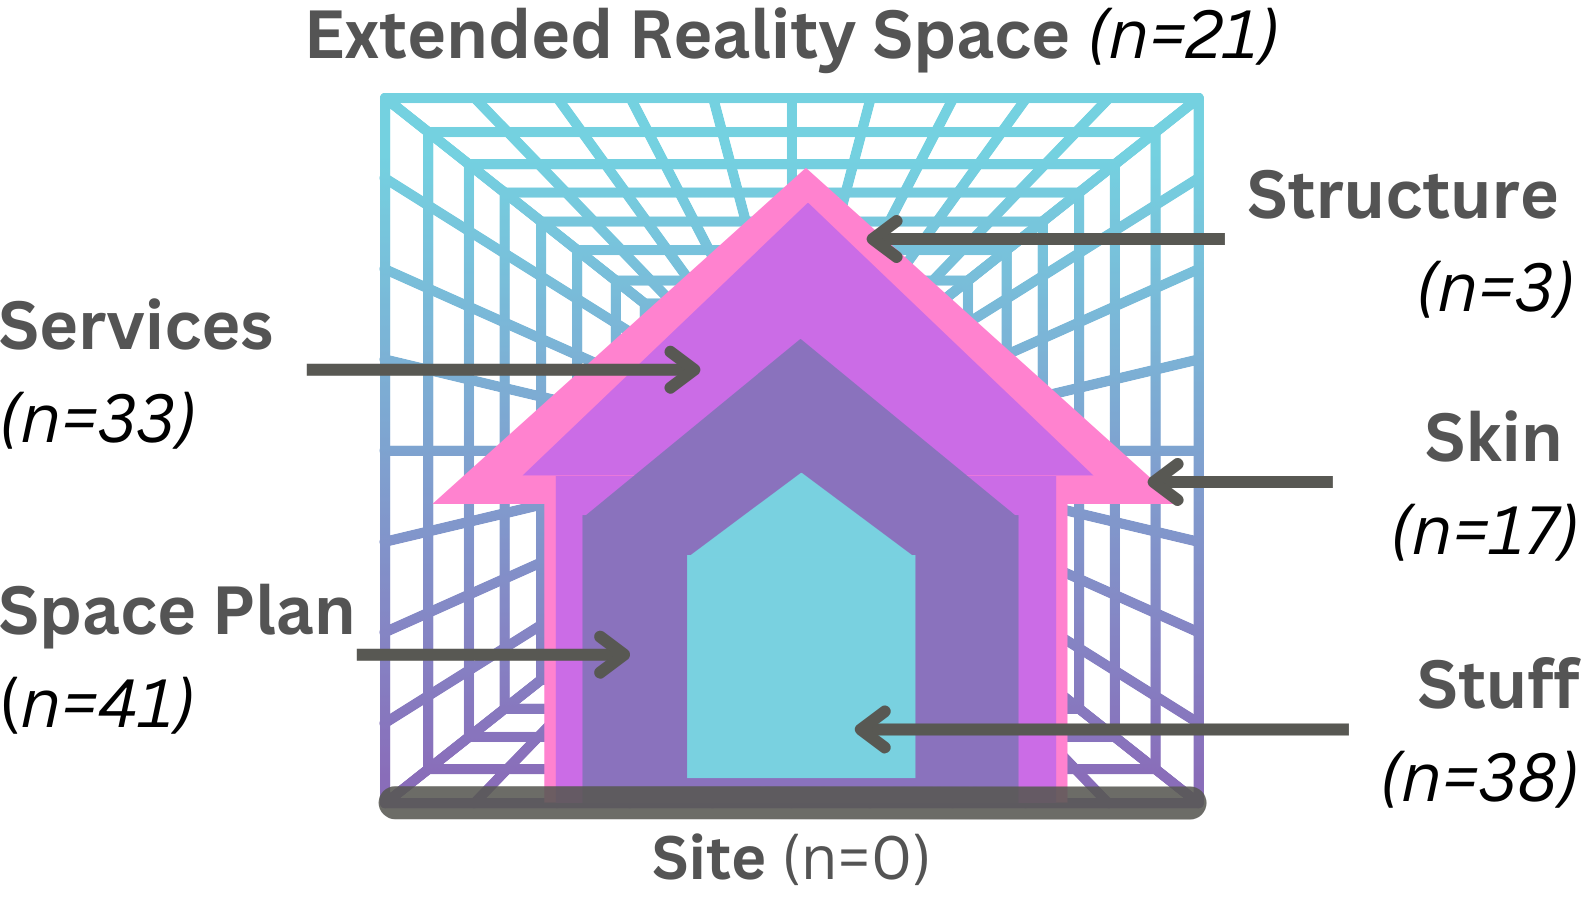
\includegraphics[width=.72\linewidth]{images/smart-building-layers.png}
    \caption{The layers of the smart building, adopted from \citet{brand1995buildings}'s shearing layers. In our scoping review, we find the \textit{Space Plan} to be the largest layer in contrast to the \textit{Site} layer that has no interventions. We additionally define the \textit{Extended Reality Space} layer to accommodate a new layer of temporality that represents the use of extended reality with smart buildings.}
    \label{fig:smart-building-layers}
\end{mainfigure}
 
\paragraph{The Temporal Layers of the Smart Building}
We also positioned technologies following  \citet{brand1995buildings}'s ``Shearing layers''  (\autoref{fig:smart-building-layers}). Brand describes six distinct layers of a building based on its temporal lifespan: \textit{Site}, \textit{Structure}, \textit{Skin}, \textit{Services}, \textit{Space Plan}, and \textit{Stuff} \cite{brand1995buildings}. The majority of interventions were concentrated in the \textit{Space Plan} (n = 41) and \textit{Stuff} (n = 38) layers. This aligns with their transient and flexible nature, making them ideal for smart building technologies and prototypes that do not require major structural changes such as smart furniture, moving walls, and interactive floors. The \textit{Services} layer (n = 33), traditionally encompassing HVAC, plumbing, and electrical systems, was reappropriated to include technologies related to occupant comfort: air quality, thermal conditions, lighting, and acoustics. 

The \textit{Skin} (n = 17) and \textit{Structure} (n = 3) layers saw fewer interventions, reflecting their enduring and foundational nature. The \textit{Skin} layer---encompassing fa\c{c}ades and exteriors---is periodically updated, but less frequently than more adaptable layers. Interventions in the \textit{Structure} layer, which includes foundations and load-bearing elements, are scarce due to the complexity and expense of altering these fundamental components. Unsurprisingly, smart building technologies tend to focus on layers that can be modified more easily, leaving structural changes largely to traditional architectural and engineering domains. 
There were no interventions categorised under the \textit{Site} layer. This absence reflects that this layer, concerned with the building's geographical location and context, falls outside the immediate focus of smart building technologies. Urban HCI work often addresses connections to the site of the building \cite{fischer2012urban}, but such considerations extend beyond the scope of our review.

To accommodate works that extend physical space using augmented and virtual means, we introduced the \textit{Extended Reality Space} (n = 21) layer. This addition reflects the growing importance of technologies that expand the physical confines of traditional building layers. Unlike traditional building layers bound by material lifespans, the \textit{Extended Reality Space} operates independently of physical constraints. It introduces a dynamic layer to building temporality, where digital and virtual environments such as AR/VR can be updated or transformed almost instantaneously. It interacts with physical elements without altering them (apart from using devices like headsets necessary to perceive virtual content), providing temporal flexibility in which both temporary and permanent digital interventions coexist. 
